\documentclass{beamer}
\usepackage{etex}
\reserveinserts{28}

\usepackage{fancyvrb}
\usepackage{color, colortbl}
\usepackage{listings}
\usepackage{url}
\usepackage{array}
\usepackage{calc}
\usepackage{ctable}
\usepackage{amsmath}
\usepackage{cite}
\usepackage{graphicx}
\usepackage{listings}
\usepackage{xspace}
\usepackage{hyperref}
\usepackage{subfigure}
\usepackage{multicol}
\definecolor{lightgray}{rgb}{0.9,0.9,0.9}



\lstset{ %
language=C++,                % choose the language of the code
basicstyle=\tiny,       % the size of the fonts that are used for the code
%numbers=left,                   % where to put the line-numbers
numbers=none,                   % where to put the line-numbers
numberstyle=\scriptsize,      % the size of the fonts that are used for the line-numbers
stepnumber=1,                   % the step between two line-numbers. If it's 1 each line will be numbered
numbersep=15pt,                  % how far the line-numbers are from the code
backgroundcolor=\color{lightgray},  % choose the background color. You must add \usepackage{color}
%backgroundcolor=none,  % choose the background color. You must add \usepackage{color}
showspaces=false,               % show spaces adding particular underscores
showstringspaces=false,         % underline spaces within strings
showtabs=false,                 % show tabs within strings adding particular underscores
frame=single,	                % adds a frame around the code
%frame=none,	                % adds a frame around the code
tabsize=2,	                % sets default tabsize to 2 spaces
%captionpos=b,                   % sets the caption-position to bottom
captionpos=n,
%basicstyle=\small,
%basicstyle=\small\sffamily,
basicstyle=\sffamily\small,
%basicstyle=\ttfamily\small,
breaklines=true,                % sets automatic line breaking
breakatwhitespace=false,        % sets if automatic breaks should only happen at whitespace
columns=fullflexible,
title=\lstname,                 % show the filename of files included with \lstinputlisting; also try caption instead of title
escapeinside={\%*}{*)},          % if you want to add a comment within your code
morekeywords={chare,mainchare,module,mainmodule,entry,readonly,array,serial,for,when,if,then,else,overlap,while,forall,threaded,sync,message,group,nodegroup},
aboveskip=2pt,
belowskip=2pt,
lineskip=0pt,
xleftmargin=1em,
xrightmargin=1em,
%xleftmargin=10pt
abovecaptionskip=0pt,
belowcaptionskip=0pt,
}

\hypersetup{
    colorlinks,%
    citecolor=black,%
    filecolor=black,%
    linkcolor=black,%
    urlcolor=magenta
}


\usefonttheme{professionalfonts}
\usetheme{Boadilla}
\usecolortheme{beaver}

%\AtBeginSubsection[]
%{
%    \begin{frame}{Outline}
%        \tableofcontents[currentsection,currentsubsection]
%    \end{frame}
%}

\AtBeginSection[]{
%  \setbeamercolor{section in toc shaded}{use=structure,fg=structure.fg}
%  \setbeamercolor{section in toc}{fg=mycolor}
%  \setbeamercolor{subsection in toc shaded}{fg=black}
%  \setbeamercolor{subsection in toc}{fg=mycolor}
  \frame<beamer>{\begin{multicols}{2}
  \frametitle{Outline}
  \setcounter{tocdepth}{2}  
%  \tableofcontents[currentsection,subsections]
  \tableofcontents[currentsection,currentsubsection]
\end{multicols} 
 }
}


\newcommand{\charm}{Charm++}
\newcommand{\code}[1]{\colorbox{lightgray}{\texttt{#1}}}
\newcommand{\transition}[1]{\begin{frame}[plain]\begin{center}\LARGE #1\end{center}\end{frame}}
\newcommand{\comment}[1]{ }
\newcommand{\eat}[1]{ }

\DefineVerbatimEnvironment{codeverb}{Verbatim}{fontsize=\small}

\let \isForClass 1
\if \isForClass 1
  \newcommand{\removeForClass}[2]{#2}
  \else
  \newcommand{\removeForClass}[2]{#1}
\fi


\title{Load Balancing in Charm++}

\author[Laxmikant V.~Kale]{
Laxmikant V.~Kale
}
\date{\today}

\begin{document}

\begin{frame}[fragile]
  \frametitle{Observations: Parallel applications}
    \begin{itemize}
    \item Obtaining best performance on parallel computers is difficult due to properties exhibited by applications 
      \begin{itemize}
        \item Multi-resolution - variation in task granularity
        \item Multi-module - loosely connected diverse tasks
        \item {\color{red} Dynamic/adaptive: to handle application variation}
        \item {\color{red} Adapt to a volatile computational environment}
        \item Exploit heterogeneous architecture - GPUs, MICs
      \end{itemize}
    \item Consequences:
      \begin{itemize}
        \item Must support automated resource management
        \item This lecture is focussed on {\color{red} load balancing}
      \end{itemize}
    \end{itemize}
\end{frame}

\begin{frame}[fragile]
  \frametitle{What is load imbalance?}
  \begin{columns}
  \begin{column}{.6\textwidth} 
  \centering
  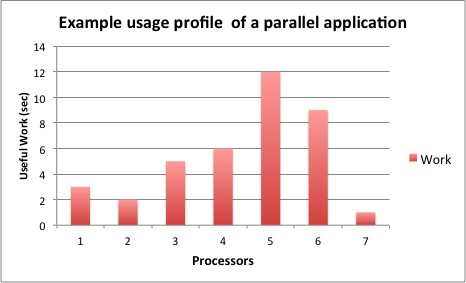
\includegraphics[width=\textwidth]{cs598lvk/diagrams/load_imbalance.jpg}
  \end{column}
  \begin{column}{.4\textwidth} 
  \begin{itemize}
  \item Application completes only when all processor finishes 
  \item Different processors gets variable work
  \item Resource wasted in waiting
  \end{itemize}
  \end{column}
  \end{columns}
\end{frame}

\begin{frame}[fragile]
  \frametitle{What is desirable?}
  \centering
  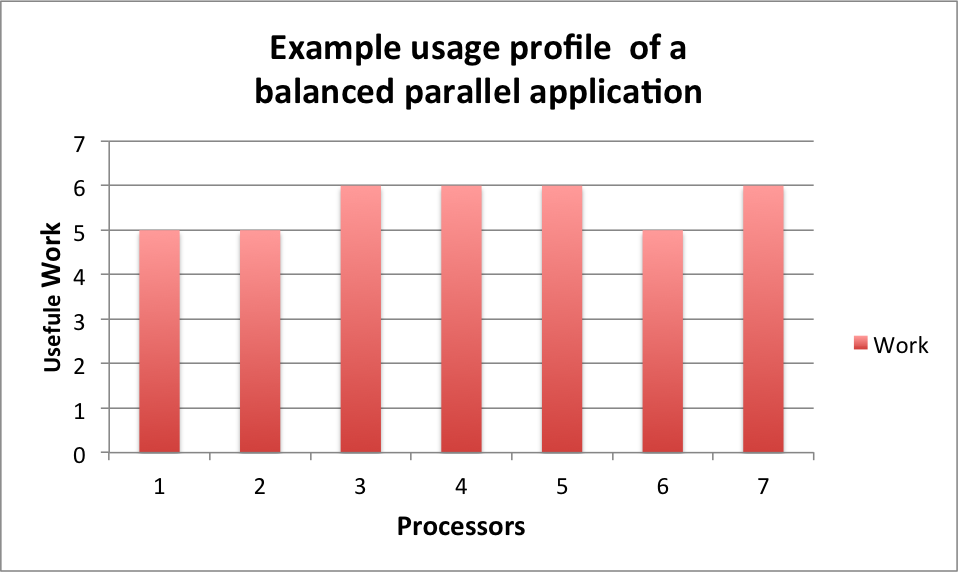
\includegraphics[width=.7\textwidth]{cs598lvk/diagrams/balanced.png}
  \begin{itemize}
  \item Work is evenly divided among processors to make best use of the available resources
  \item How - Static and Dynamic Load balancing
  \end{itemize}
\end{frame}

\begin{frame}[fragile]
  \frametitle{Static Mapping for Load Balancing}
    \begin{itemize}
      \item In some applications, load pattern does not change much as computation progresses
      \begin{itemize}
        \item You, the programmer, may want to control which chare lives on which processors
        \item This is also true when  load may evolve over time, but you want to control initial placement of chares
      \end{itemize}
      \item The feature in Charm++ for this purpose is called \textbf{Map
      Objects}
      \item Sec. 13.2.2 of the Charm++ manual
    \end{itemize}
\end{frame}

\begin{frame}[fragile]
    \frametitle{CkArrayOptions - customizing array creation}
    \begin{itemize}
      \item To specify static initial mapping, we must first learn this feature
      \begin{itemize}
        \item Whenever a chare array is created, one can pass an optional
        parameter of type CkArrayOptions
      \end{itemize}
    \end{itemize}
      \begin{lstlisting}
      CkArrayOptions opts(numElements); //array to be created with numElements chares
      //set other properties of opts (discussed later in the course)
      P = CProxy_A::CkNew(parameters, opts);
      \end{lstlisting}
    \begin{itemize}
      \item Many propperties of arrays can be set using this method.
      \item {\color{red} In particular, we can specify a map object}
    \end{itemize}
\end{frame}

\begin{frame}[fragile]
    \frametitle{CkArrayMap - base class of all map objects}
    \begin{lstlisting}
    class CkArrayMap : public Group
    {
      public:
      //......
      
      //Return the processor number for this element of this array
      virtual int procNum(int arrayHdl, const CkArrayIndex element);

      //Return an ``arrayHdl'', given some information about the array
      virtual int registerArray(CkArrayIndex numElements, CkArrayID aid);
    }
    \end{lstlisting}
    \begin{itemize}
    \item If you want to specify a map for a chare array you are about to
    create, you must first define a subclass of CkArrayMap
    \item It is a “Group”.. More on that much later
    \item You don’t need to know any more than inheriting from it for now
    \end{itemize}
\end{frame}

\begin{frame}[fragile]
    \frametitle{Defining your own map}
    \begin{lstlisting}
     class BlockMap : public CkArrayMap
     { public:
       BlockMap(void) {}
       BlockMap(CkMigrateMessage *m){}

       // place elements in blocks of 32
       int procNum(int /*arrayHdl*/,const CkArrayIndex& idx) {
           int elem=*(int *)idx.data();
           int penum =  (elem/32) % CkNumPes();
           return penum;
       }
       int registerArray(CkArrayIndex& numElements,CkArrayID aid) 
       { return 0; }
     };
    \end{lstlisting}
    \begin{itemize}
        \item \texttt{CkArrayIdx} is a datatye that’s normally used by the system. You
        can peek into it to extract indices. The example works for 1D array
    \end{itemize}
\end{frame}

\begin{frame}[fragile]
    \frametitle{Putting them alll together}
    \begin{lstlisting}
      //Create the map group
      CProxy_BlockMap myMap=CProxy_BlockMap::ckNew();
      //Make a new array using that map
      CkArrayOptions opts(nElements);
      opts.setMap(myMap);
      a1=CProxy_A1::ckNew( parameters,opts);
    \end{lstlisting}
    \begin{itemize}
    \item Create a map object, 
    \item pass it to an \texttt{CkArrayOptions} object (opts here), and then 
    \item pass that to \texttt{ckNew}
    \end{itemize}
\end{frame}

\begin{frame}[fragile]
    \frametitle{Why is CkArrayMap an object}
    \begin{itemize}
      \item It looks like a function.. Given an index, return a PE (processor
      number)
      \item In many simple cases, that is enough
      \item In general, you may want to remember some data in state information, so you can construct the answer quickly
      \item The system may ask you for this information at creation, but also later during method invocation
    \end{itemize}
\end{frame}

\begin{frame}[fragile]
    \frametitle{Exercises}
    \begin{itemize}
        \item Write a map object for cyclic distribution of a 1D chare array
        \item Write a map object for a 2D chare array in a block fashion, ensuring that they are not heavily load imbalanced, even when running on non-square number of processors
        \begin{itemize}
            \item Should work for any combination of array sizes and number of processors
        \end{itemize}
        \item Extend the previous one for the case where each processor has a x,y,z coordinate (the physical network is a torus, for example)
    \end{itemize}
\end{frame}

\begin{frame}[fragile]
\frametitle{Chare Migration: motivations}
\begin{itemize}
\item Chares are initially placed according to a placement map
\begin{itemize}
\item The user can specify this map
\end{itemize}
\item While running, some processors might be overloaded
\begin{itemize}
\item Need to rebalance the load
\end{itemize}
\item Automatic checkpoint
\begin{itemize}
\item Migration to disk
\end{itemize}
\item Chares are made serializable for transport using the Pack UnPack (PUP) framework
\end{itemize}
\end{frame}

\begin{frame}[fragile]
\frametitle{The PUP Process}
  \begin{center}
    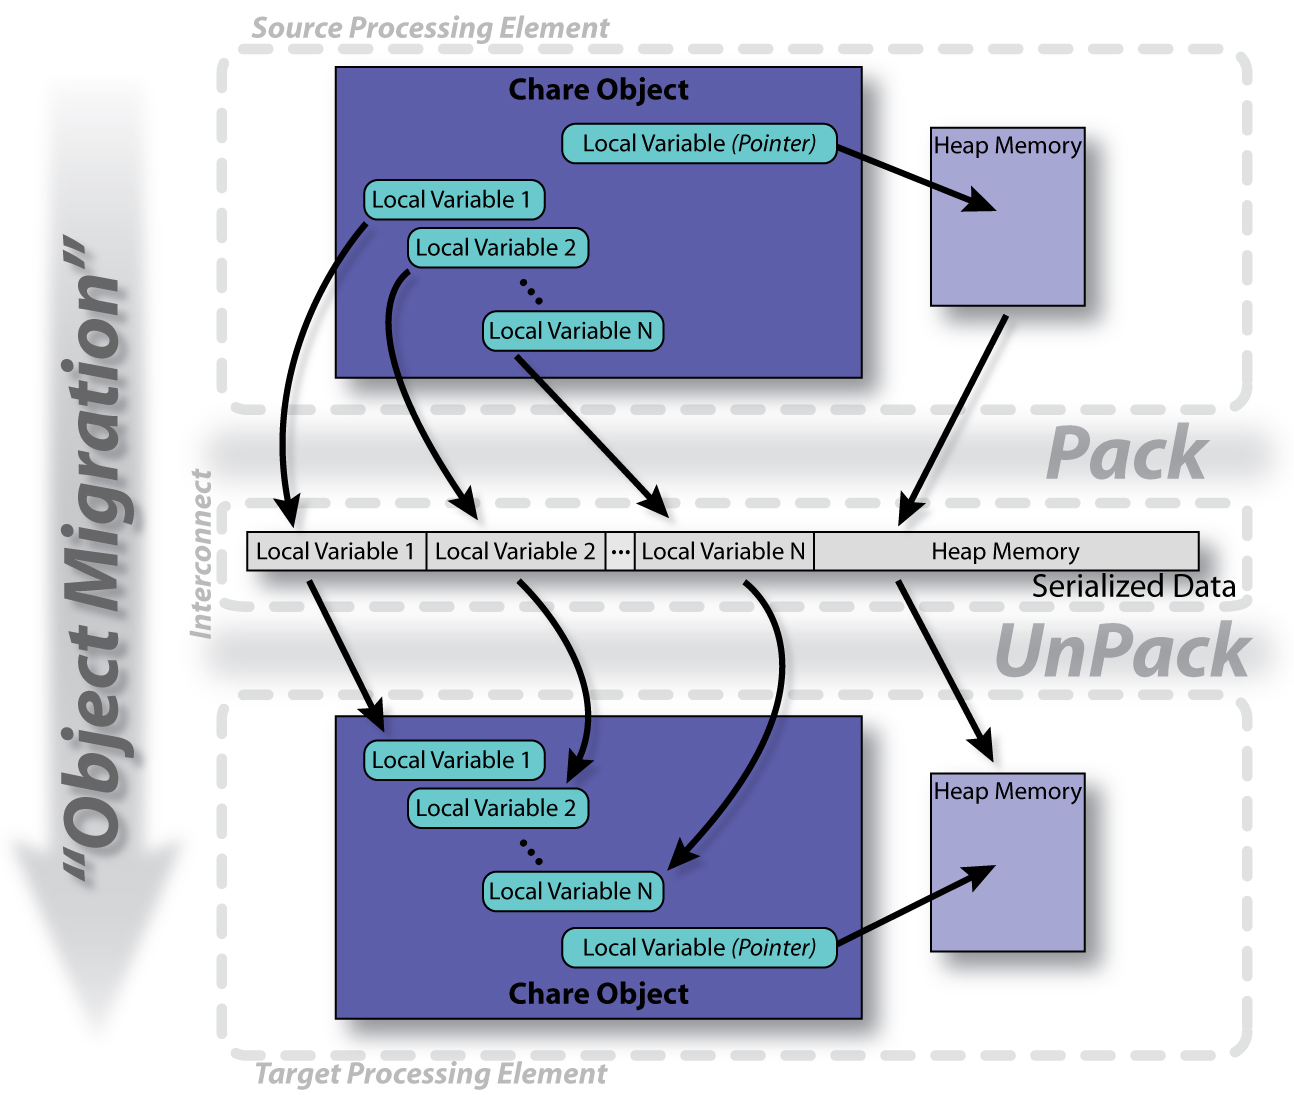
\includegraphics[width=0.8\textwidth]{figures/PUPProcess.png}
  \end{center}
\end{frame}


% \begin{frame}[fragile]
% \frametitle{PUP Usage Sequence}
%   \begin{center}
%     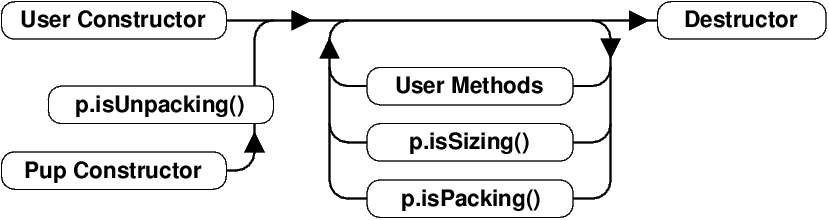
\includegraphics[width=0.8\textwidth]{figures/PUPUsage.png}
%   \end{center}
% \begin{columns}
%  \begin{column}{0.5\textwidth}
%  \begin{itemize}
%  \item Migration out:
%  \begin{itemize}
%  \item ckAboutToMigrate
%  \item Sizing
%  \item Packing
%  \item Destructor
%  \end{itemize}
%  \end{itemize}
%  \end{column}
%  \begin{column}{0.5\textwidth}
%  \begin{itemize}
%  \item Migration in:
%  \begin{itemize}
%  \item Migration constructor
%  \item UnPacking
%  \item ckJustMigrated
%  \end{itemize}
%  \end{itemize}
% \end{column}
% \end{columns}
% \end{frame}

\begin{frame}[fragile]
\frametitle{Writing a PUP routine}
 \begin{columns}
 \begin{column}{0.5\textwidth}
   \begin{lstlisting}
class MyChare : public CBase_MyChare {
  int a;   float b;   char c;
  float localArray[LOCAL_SIZE];
};
 \end{lstlisting}
 \end{column}
 \begin{column}{0.5\textwidth}
  \begin{lstlisting}
void pup(PUP::er &p) {
   CBase_MyChare::pup(p);
   p | a;  p | b; p | c;
}
  \end{lstlisting}
  \end{column}
  \end{columns}
\end{frame}

\begin{frame}[fragile]
\frametitle{Writing a PUP routine}
 \begin{columns}
 \begin{column}{0.5\textwidth}
   \begin{lstlisting}
class MyChare : public CBase_MyChare {
  int a;   float b;   char c;
  float localArray[LOCAL_SIZE];
  int heapArraySize;
  float* heapArray;
  MyClass *pointer;
 
  public:
   MyChare();
   MyChare(CkMigrateMessage *msg) {};
   ~MyChare() {
     if (heapArray != NULL) {
       delete [] heapArray;
       heapArray = NULL;
     }
};
 \end{lstlisting}
 \end{column}
 \begin{column}{0.5\textwidth}
  \begin{lstlisting}
void pup(PUP::er &p) {
   CBase_MyChare::pup(p);
   p | a;  p | b; p | c;
   p(localArray, LOCAL_SIZE);
   p | heapArraySize;
   if (p.isUnpacking()) {
     heapArray = new float[heapArraySize];
   }
   p(heapArray, heapArraySize);
   int isNull = (pointer==NULL) ? 1 : 0;
   p | isNull;
   if (!isNull) {
     if (p.isUnpacking()) pointer = new MyClass();
     p | *pointer;
   }
 }
}
  \end{lstlisting}
  \end{column}
  \end{columns}
\end{frame}


\begin{frame}[fragile]
\frametitle{PUP: Concerns}
\begin{itemize}
\item If variables are added to an object, update the PUP routine
\item If the object allocates data on the heap, copy it recursively, not just the pointer
\item Remember to allocate memory while unpacking
\item Sizing, Packing, and Unpacking must scan the variables in the same order
\item Test PUP routines with “+balancer RotateLB”
\end{itemize}
\end{frame}

\transition{Dynamic Load Balancing}

\begin{frame}[fragile]
\frametitle{How to Diagnose Load Imbalance}
\begin{itemize}
 \item Often hidden in statements such as:
 \begin{itemize}
  \item Very high synchronization overhead
  \begin{itemize}
   \item Most processors are waiting at a reduction
  \end{itemize}
 \end{itemize}
 \item Count total amount of computation (ops/flops) per processor
 \begin{itemize}
  \item In each phase! 
  \item Because the balance may change from phase to phase
 \end{itemize}
\end{itemize}
\end{frame}

\begin{frame}[fragile]
\frametitle{Golden Rule of Load Balancing}
\emph{Fallacy: objective of load balancing is to minimize variance in load across processors}

\begin{itemize}
 \item[]\emph{Example:}
 \begin{itemize}
  \item  50,000 tasks of equal size, 500  processors:
  \begin{itemize}
   \item A: All processors get 99, except last 5 gets $100+99 = 199$
   \item OR, B:  All processors have 101, except last 5 get 1
  \end{itemize}
 \end{itemize}
 \item[] Identical variance, but situation A is much worse!
\end{itemize}


\emph{Golden Rule: It is ok if a few processors idle, but avoid having processors that are overloaded with work}


\emph{Finish time} = $max_i$(Time on processor $i$)
\begin{itemize}
\item[] excepting data dependence and communication overhead issues
\end{itemize}

The speed of any group is the speed of slowest member of that group.
\end{frame}

\begin{frame}[fragile]
\frametitle{Automatic Dynamic Load Balancing}
\begin{itemize}
\item Measurement based load balancers
\begin{itemize}
\item Principle of persistence: In many CSE applications, computational loads and communication patterns tend to persist, even in dynamic computations
\item Therefore, recent past is a good predictor of near future
\item Charm++ provides a suite of load-balancers 
\item Periodic measurement and migration of objects
\end{itemize}
\item Seed balancers (for task-parallelism)
\begin{itemize}
\item Useful for divide-and-conquer and state-space-search applications
\item Seeds for charm++ objects moved around until they take root
\end{itemize}
\end{itemize}
\end{frame}

\begin{frame}[fragile]
\frametitle{Using the Load Balancer}
\begin{itemize}
\item link a LB module 
\begin{itemize}
\item \code{-module <strategy>}
\item RefineLB, NeighborLB, GreedyCommLB, others…
\item EveryLB will include all load balancing strategies
\end{itemize}
\item compile time option (specify default balancer)
\begin{itemize}
\item \code{-balancer RefineLB}
\item runtime option
\item \code {+balancer RefineLB}
\end{itemize}
\end{itemize}
\end{frame}

\begin{frame}
\frametitle{Code to Use Load Balancing}
\begin{itemize}
\item Insert \code{if (myLBStep) AtSync() else ResumeFromSync();} call at natural barrier
\item Implement \code{ResumeFromSync()} to resume execution
\begin{itemize}
\item Typical ResumeFromSync contribute to a reduction
\end{itemize}
\end{itemize}
\end{frame}

\begin{frame}[fragile]
\frametitle{Example: Stencil}
\begin{lstlisting}[basicstyle=\tiny]
while (!converged) {
  serial {
    int x = thisIndex.x, y = thisIndex.y, z = thisIndex.z;
    copyToBoundaries();
    thisProxy(wrapX(x-1),y,z).updateGhosts(i, RIGHT, dimY, dimZ, right);
    /* ...similar calls to send the 6 boundaries... */
    thisProxy(x,y,wrapZ(z+1)).updateGhosts(i, FRONT, dimX, dimY, front);
  }
  for (remoteCount = 0; remoteCount < 6; remoteCount++) {
    when updateGhosts[i](int i, int d, int w, int h, double b[w*h])
    serial { updateBoundary(d, w, h, b); }
  }
  serial {
    int c = computeKernel() < DELTA;
    CkCallback cb(CkReductionTarget(Jacobi, checkConverged), thisProxy);
    if (i%5 == 1) contribute(sizeof(int), \&c, CkReduction::logical_and, cb);
  }
  if (i % lbPeriod == 0) { serial { AtSync(); } when ResumeFromSync() {} }
  if (++i % 5 == 0) {
    when checkConverged(bool result) serial {
      if (result) { mainProxy.done(); converged = true; }
    }
  }
}
\end{lstlisting}
\end{frame}

\begin{frame}
\frametitle{Performance}
\begin{centering}
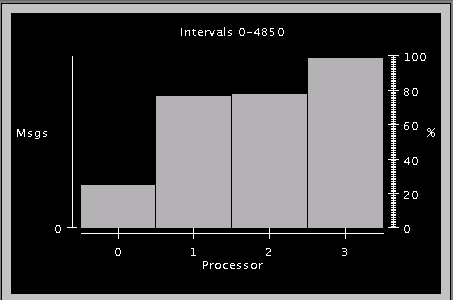
\includegraphics[width=0.5\textwidth]{figures/beforeLB}
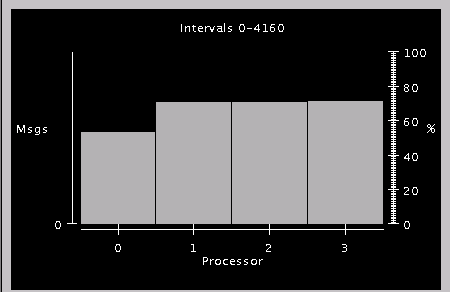
\includegraphics[width=0.5\textwidth]{figures/afterLB}
\end{centering}
\end{frame}

%\begin{frame}[fragile]
%\frametitle{Grainsize and Load Balancing}
%\begin{itemize}
%\item[] How Much Balance Is Possible?
%\end{itemize}
%\begin{columns}
%  \begin{column}[T]{2.8in}
%  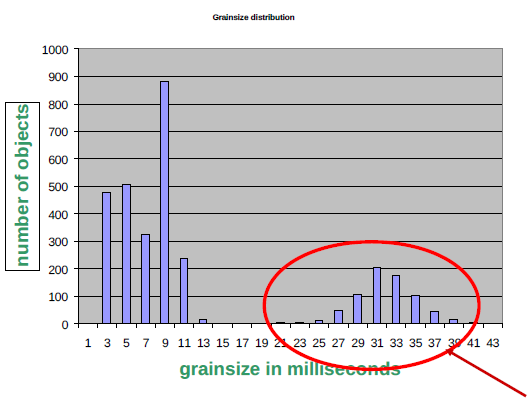
\includegraphics[width=2.8in, height=2.0in]{figures/histogramGrains}
%  \end{column}
%
%  \begin{column}[T]{5cm}
%  Solution:\\ 
%  Split compute objects that may have too much work,
%  using a heuristic based on number of interacting atoms
%  \end{column}
%\end{columns}
%\end{frame}

%\begin{frame}[fragile]
%\frametitle{Grainsize For Extreme Scaling}
%\begin{itemize}
% \item Strong Scaling is limited by expressed parallelism
% \begin{itemize}
%  \item Minimum iteration time limited by lengthiest computation
%  \begin {itemize} 
%    \item Largest grains set lower bound
%  \end{itemize}
% \end{itemize}
% \item 1-away generalized to k-away provides fine granularity control
%\end{itemize}
%\begin{centering}
%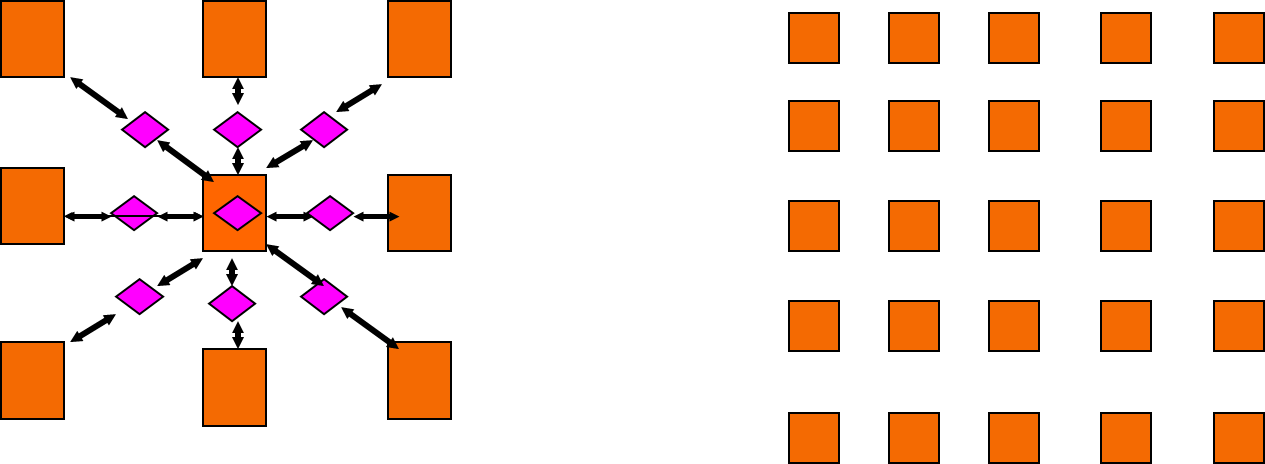
\includegraphics[width=1.0\textwidth]{figures/1away2away}
%\end{centering}
%\end{frame}
%
%\begin{frame}[fragile]
%\frametitle{NAMD: 2-AwayX Example}
%\begin{centering}
%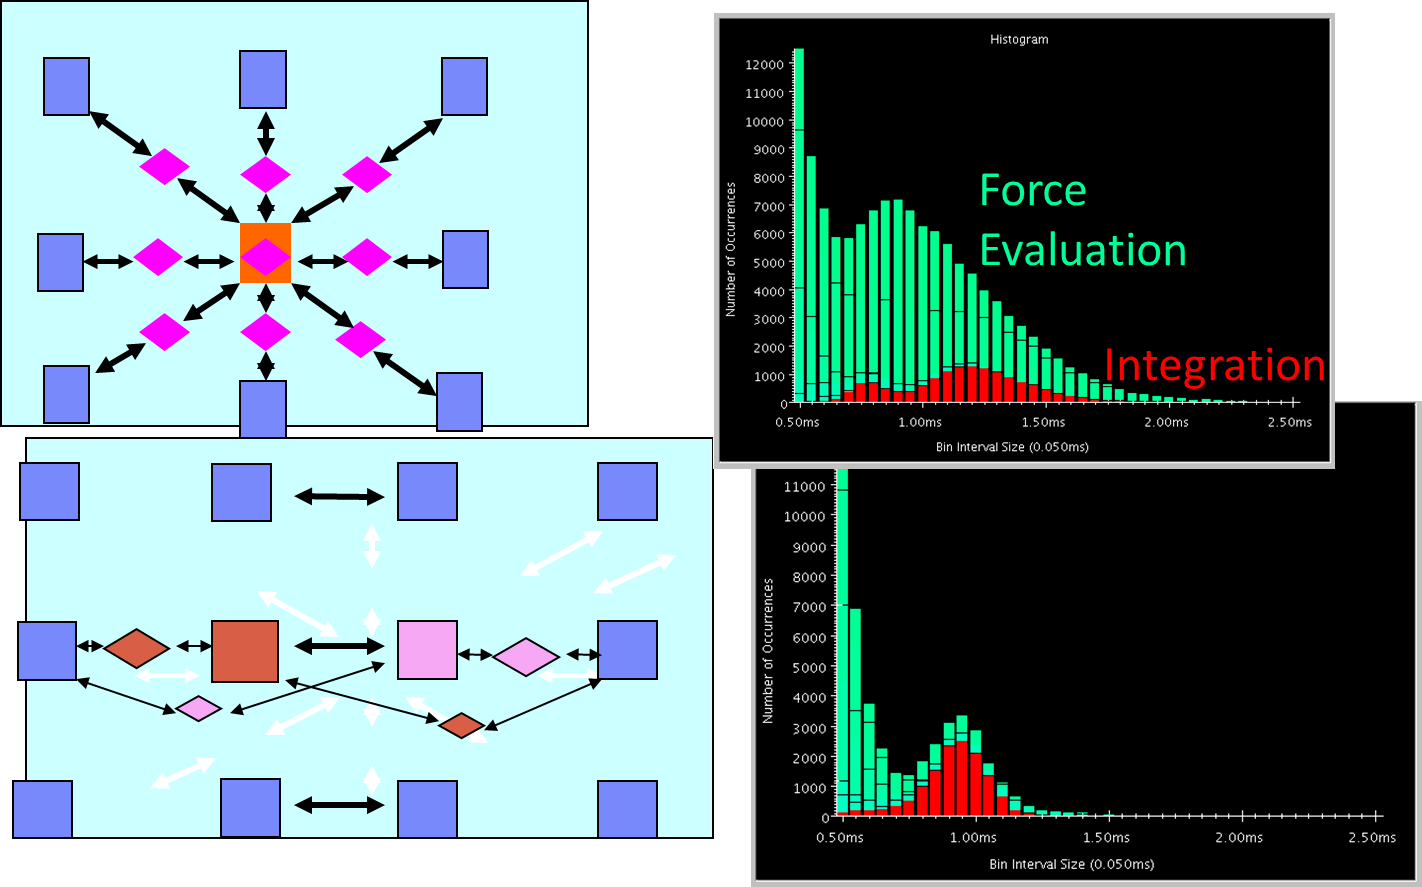
\includegraphics[width=1.0\textwidth]{figures/2awayDiagramPlusHistos}
%\end{centering}
%\end{frame}
%
\begin{frame}[fragile]
\frametitle{Load Balancing Strategies}
\begin{itemize}
 \item Classified by when it is done:
 \begin{itemize}
  \item Initially
  \item Dynamic: Periodically
  \item Dynamic: Continuously
 \end{itemize}
 \item Classified by whether decisions are taken with global information
 \begin{itemize}
  \item Fully centralized
  \begin{itemize}
   \item Quite good a choice when load balancing period is high
  \end{itemize}
 \item Fully distributed
 \begin{itemize}
  \item Each processor knows only about a constant number of neighbors
  \item Extreme case: totally local decision (send work to a random destination processor, with some probability).
 \end{itemize}
\item Use \emph{aggregated} global  information, and \emph{detailed} neighborhood info.
\end{itemize}
\end{itemize}
\end{frame}

\begin{frame}[fragile]
\frametitle{Dynamic Load Balancing Scenarios}
\begin{itemize}
 \item Examples representing typical classes of situations
 \begin{itemize}
  \item Particles distributed over simulation space
  \begin{itemize}
   \item Dynamic: because Particles move.
   \item Cases:\\
   Highly non-uniform distribution (cosmology)\\
   Relatively Uniform distribution 
   %\begin{description}[parskip]
   %\item Highly non-uniform distribution (cosmology)
   %\item Relatively Uniform distribution 
   %\end{description}
  \end{itemize}
 \end{itemize}
\item Structured grids, with dynamic refinements/coarsening
\item Unstructured grids with dynamic refinements/coarsening
\end{itemize}
\end{frame}

%\begin{frame}[fragile]
%\frametitle{Example Case: Particles}
% Orthogonal Recursive Bisection (ORB)
% %should wrapfig the little diagram here
% \begin{itemize} 
%  \item At each stage: divide Particles equally
%  \item Processor don’t need to be a power of 2:
%  \begin{itemize} 
%   \item Divide in proportion 
%   \begin{itemize} 
%    \item 2:3 with 5 processors
%   \end{itemize}
%  \end{itemize}
% \item How to choose the dimension along which to cut?
% \begin{itemize} 
%  \item Choose the longest one
% \end{itemize}
% \item How to draw the line?
% \begin{itemize} 
%  \item All data on one processor? Sort along each dimension
%  \item Otherwise: run a distributed histogramming algorithm to find the line, recursively
% \end{itemize}
% \item Find the entire tree, and then do all data movement at once
% \begin{itemize} 
%  \item Or do it in two-three steps.
%  \item But no reason to redistribute particles after drawing each line.
% \end{itemize}
%\end{itemize}
%\end{frame}

\begin{frame}[fragile]
\frametitle{Dynamic Load Balancing using Objects}

Object based decomposition (I.e. virtualized decomposition) helps
\begin{itemize}
 \item Allows RTS to remap them to balance load
 \item But how does the RTS decide where to map objects?
 \item Just move objects away from overloaded processors to underloaded processors
 \item How is load determined?
\end{itemize}
\end{frame}

\begin{frame}[fragile]
\frametitle{Measurement Based Load Balancing}
\begin{itemize}
 \item \emph{Principle of Persistence}
 \begin{itemize}
  \item Object communication patterns and computational loads tend to persist over time
  \item In spite of dynamic behavior
  \begin{itemize}
   \item Abrupt but infrequent changes
   \item Slow and small changes
  \end{itemize}
 \end{itemize}
\item Runtime instrumentation
\begin{itemize}
 \item Measures communication volume and computation time
\end{itemize}
\item Measurement based load balancers
\begin{itemize}
 \item Use the instrumented data-base periodically to make new decisions
 \item Many alternative strategies can use the database
\end{itemize}
\end{itemize}
\end{frame}

\begin{frame}[fragile]
\frametitle{Periodic Load Balancing}

Centralized strategies:
\begin{itemize}
 \item Charm RTS collects data (on one processor) about:
 \begin{itemize}
  \item Computational Load and Communication for each pair
 \end{itemize}
 %\item If you are not using AMPI/Charm, you can do the same instrumentation and data collection
 \item Partition the graph of objects across processors
 \begin{itemize}
  \item Take communication into account
  \begin{itemize}
   \item Pt-to-pt, as well as multicast over a subset
   \item As you map an object, add to the load on both sending and receiving processor
  \end{itemize}
  \item Multicasts to multiple co-located objects are effectively the cost of a single send
 \end{itemize}
\end{itemize}
\end{frame}

\begin{frame}[fragile]
\frametitle{Typical Load Balancing Steps}
\begin{centering}
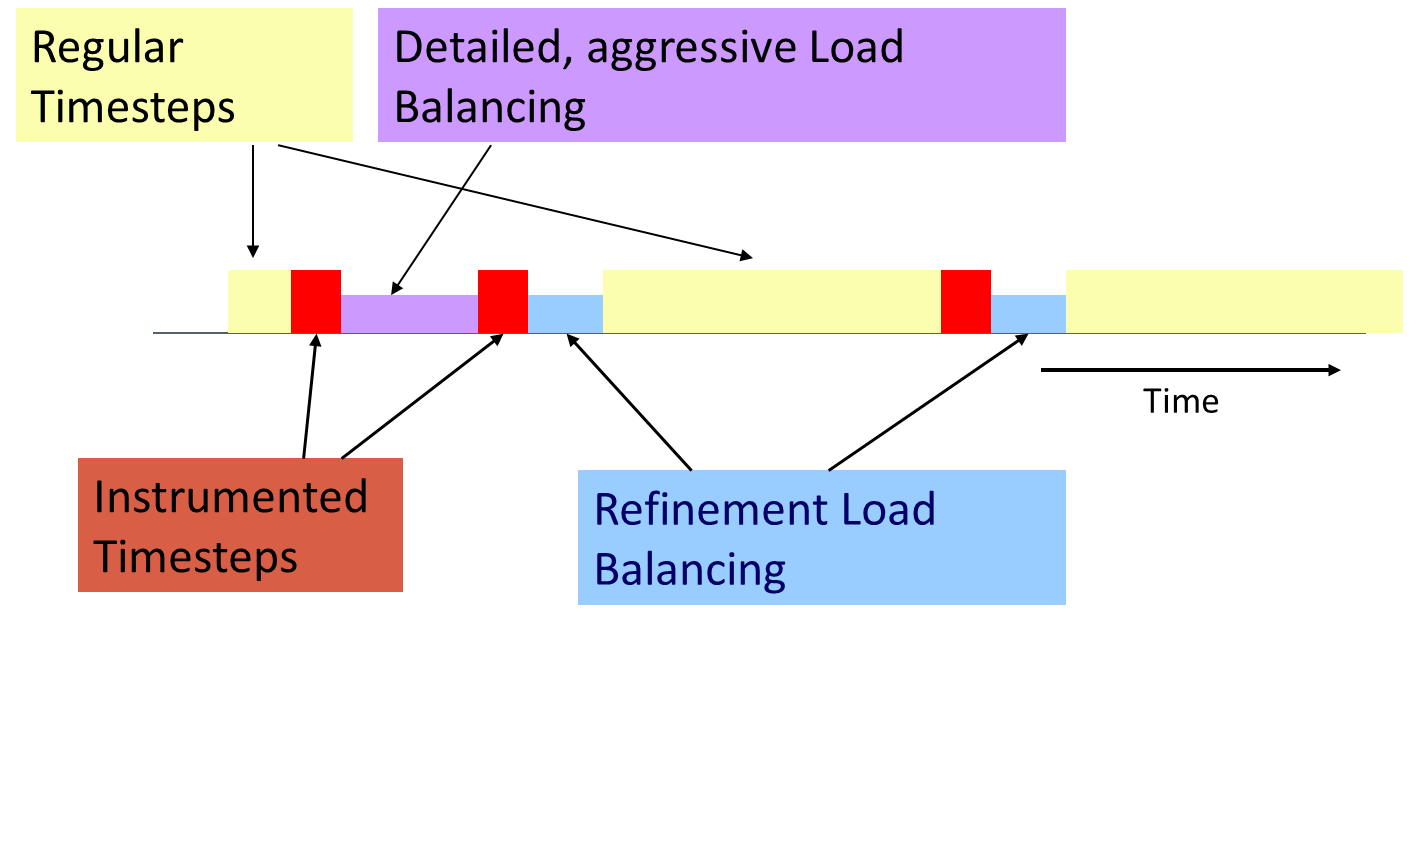
\includegraphics[width=1.0\textwidth]{figures/LBStepsDiagram}
\end{centering}
\end{frame}

% \begin{frame}[fragile]
% \frametitle{Object Partitioning Strategies}
% \begin{itemize}
%  \item You can use graph partitioners like METIS, K-R
%  \begin{itemize}
%   \item BUT: graphs are smaller, and optimization criteria are different
%  \end{itemize}
%  \item Greedy strategies:
%  \begin{itemize}
%   \item If communication costs are low: use a simple greedy strategy
%   \begin{itemize}
%    \item Sort objects by decreasing load
%    \item Maintain processors in a heap (by assigned load)
%    \item In each step: \\
%    %\begin{description}
%    % \item 
%    assign the heaviest remaining object to the least loaded processor
%    %\end{description}
%   \end{itemize}
%   \item With small-to-moderate communication cost:
%   \begin{itemize}
%    \item Same strategy, but add communication costs as you add an object to a processor
%   \end{itemize}
%   \item Always add a refinement step at the end:
%   \begin{itemize}
%    \item Swap work from heaviest loaded processor to ``some other processor''
%    \item Repeat a few times or until no improvement 
%   \end{itemize}
%  \end{itemize}
% \end{itemize}
% \end{frame}


% \begin{frame}[fragile]
% \frametitle{Object Partitioning Strategies 2}
% When communication cost is significant:
% \begin{itemize}
%  \item Still use greedy strategy, but:
%  \begin{itemize}
%   \item At each assignment step, choose between assigning O to least loaded processor and the processor that already has objects that communicate most with O.
%   \begin{itemize}
%    \item Based on the degree of difference in the two metrics
%    \item Two-stage assignments:\\
%     In early stages,  consider communication costs as long as the processors are
%     in the same (broad) load “class”,\\
%     In later stages, decide based on load
%   \end{itemize}
%  \end{itemize}
% \end{itemize}
% Branch-and-bound
% \begin{itemize}
%  \item Searches for optimal, but can be stopped after a fixed time
% \end{itemize}
% \end{frame}

\begin{frame}[fragile]
\frametitle{Crack Propagation}
\begin{centering}
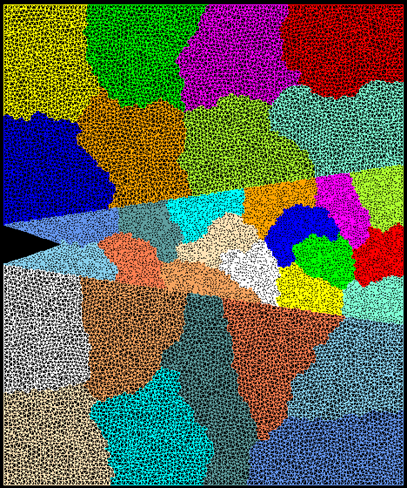
\includegraphics[width=0.4\textwidth]{figures/chunkGraph16}
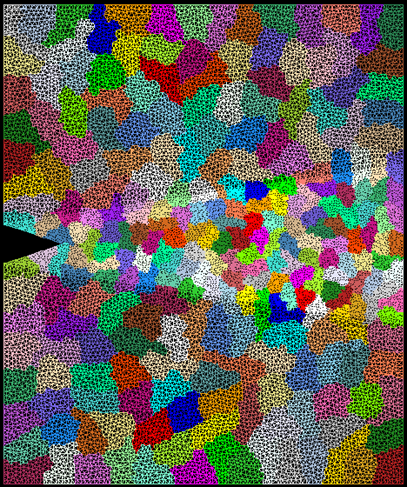
\includegraphics[width=0.4\textwidth]{figures/chunkGraph128}
\end{centering}
Decomposition into 16 chunks (left) and 128 chunks, 8 for each PE (right). The middle area contains cohesive elements. Both decompositions obtained using Metis. Pictures: S. Breitenfeld, and P. Geubelle

As computation progresses, crack propagates, and new elements are added, leading to more complex computations in some chunks
\end{frame}

\begin{frame}[fragile]
\frametitle{Load Balancing Crack Propagation}
\begin{centering}
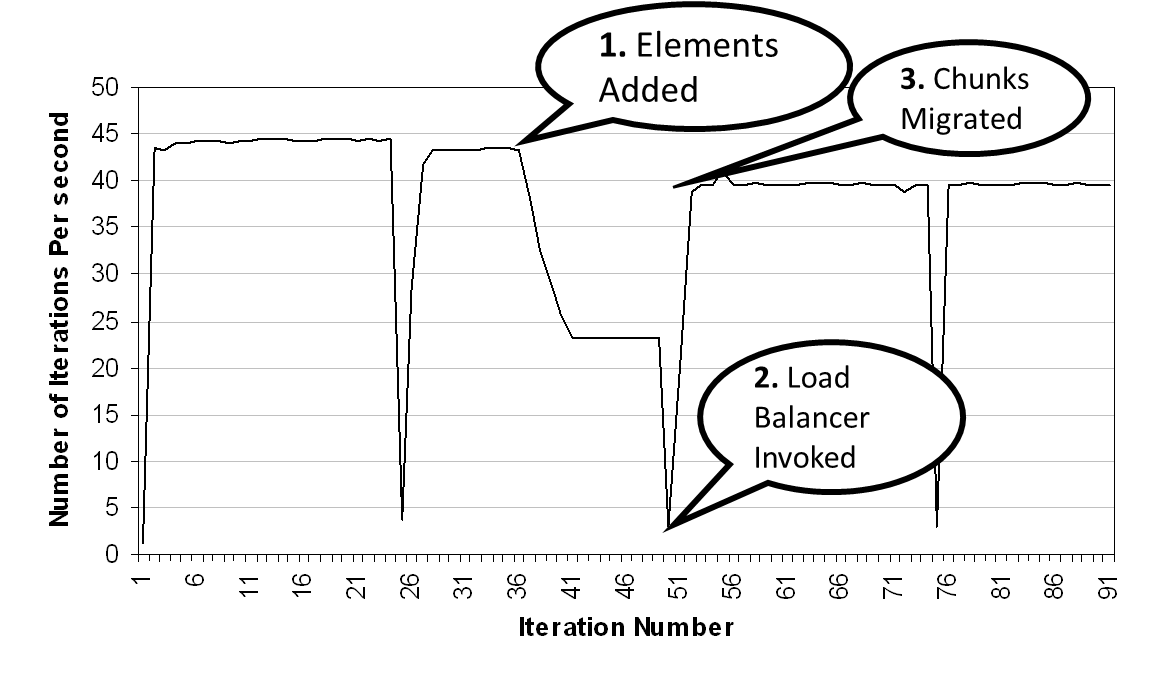
\includegraphics[width=1.0\textwidth]{figures/LButilizationCrackPropWithAnnotation}
\end{centering}
\end{frame}


\begin{frame}[fragile]
\frametitle{Distributed Load balancing}
\begin{itemize}
 \item Centralized strategies
 \begin{itemize}
  \item Still ok for 3000 processors for NAMD
 \end{itemize}
 \item Distributed balancing is needed when:
 \begin{itemize}
  \item Number of processors is large and/or 
  \item load variation is rapid
 \end{itemize}
 \item Large machines: 
 \begin{itemize}
  \item Need to handle locality of communication
  \begin{itemize}
   \item Topology sensitive placement
  \end{itemize}
  \item Need to work with scant global information
  \begin{itemize}
   \item Approximate or aggregated global information (average/max load)
   \item Incomplete global info (only “neighborhood”)
   \item Work diffusion strategies (1980s work by Kale and others!)
  \end{itemize}
  \item Achieving global effects by local action…
 \end{itemize}
\end{itemize}
\end{frame}

\begin{frame}[fragile]
\frametitle{Load Balancing on Large Machines}
\begin{itemize}
 \item Centralized load balancing strategies don’t scale on extremely large machines
 \item Limitations of centralized strategies:
 \begin{itemize}
  \item Central node: memory/communication bottleneck
  \item Decision-making algorithms tend to be very slow
 \end{itemize}
 \item Limitations of distributed strategies:
 \begin{itemize}
  \item Difficult to achieve well-informed load balancing decisions
 \end{itemize}
\end{itemize}
\end{frame}


\begin{frame}[fragile]
\frametitle{Simulation Study - Memory Overhead}
lb\_test experiments performed with the performance simulator BigSim
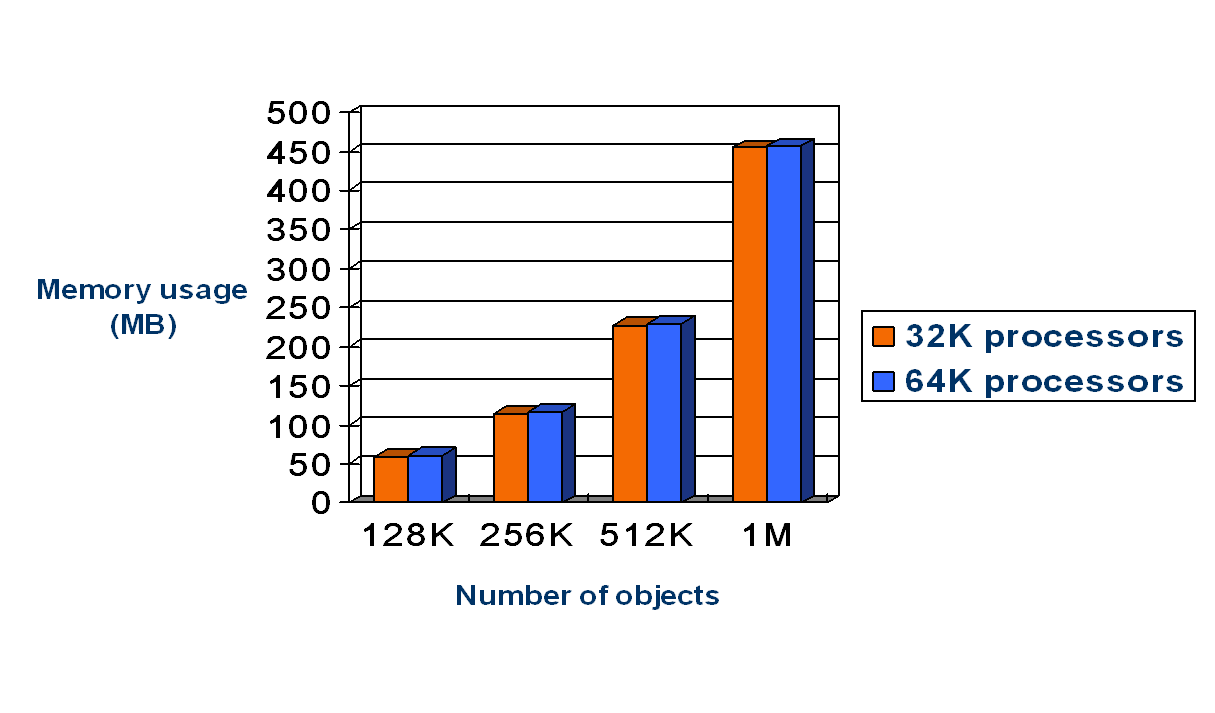
\includegraphics[width=1.0\textwidth]{figures/LBMemOverhead}
\begin{itemize}
 \item lb\_test benchmark is a parameterized program that creates a 
specified number of communicating objects in 2D-mesh.
\end{itemize}
\end{frame}


\begin{frame}[fragile]
\frametitle{Hierarchical Load Balancers}
\begin{itemize}
\item Partition processor allocation into processor groups
\item Apply different strategies at each level
\item Scalable to a large number of processors
\end{itemize}
\end{frame}

\begin{frame}[fragile]
\frametitle{Our Hybrid Scheme}
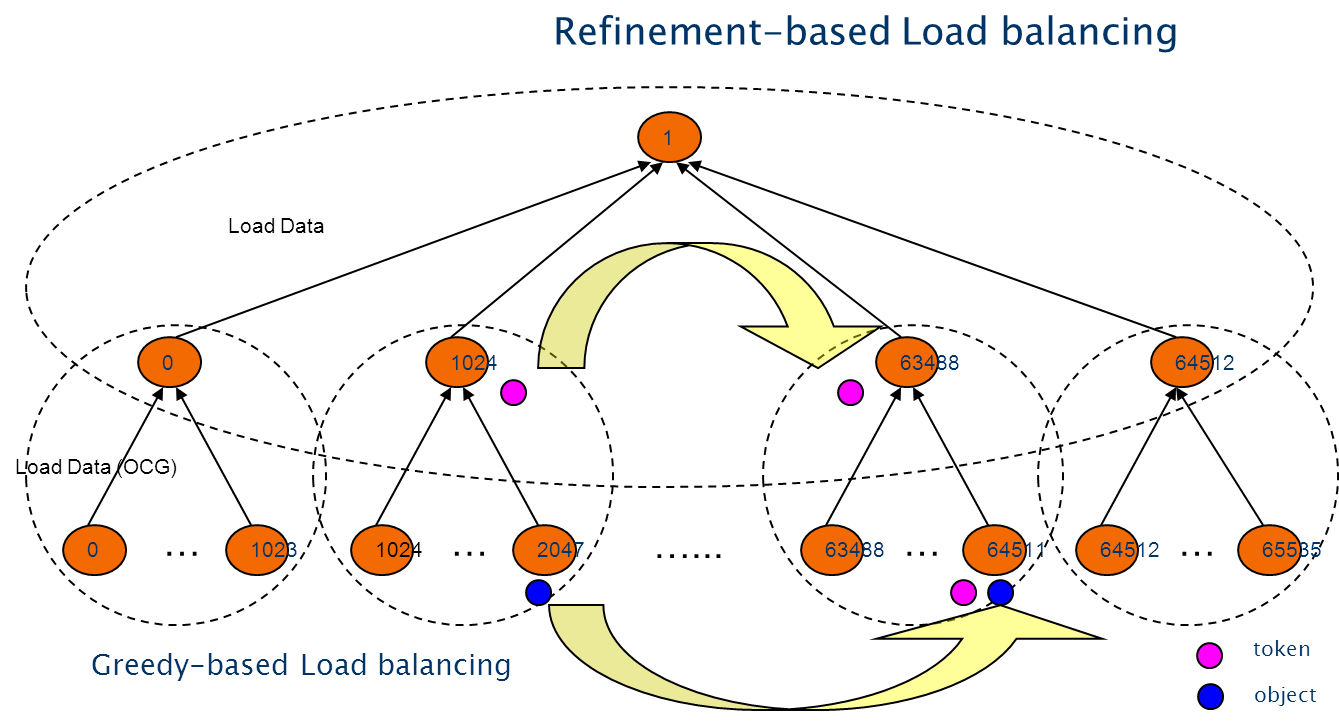
\includegraphics[width=1.0\textwidth]{figures/hybridLBScheme}
\end{frame}

\begin{frame}[fragile]
\frametitle{Hybrid Load Balancing Performance}
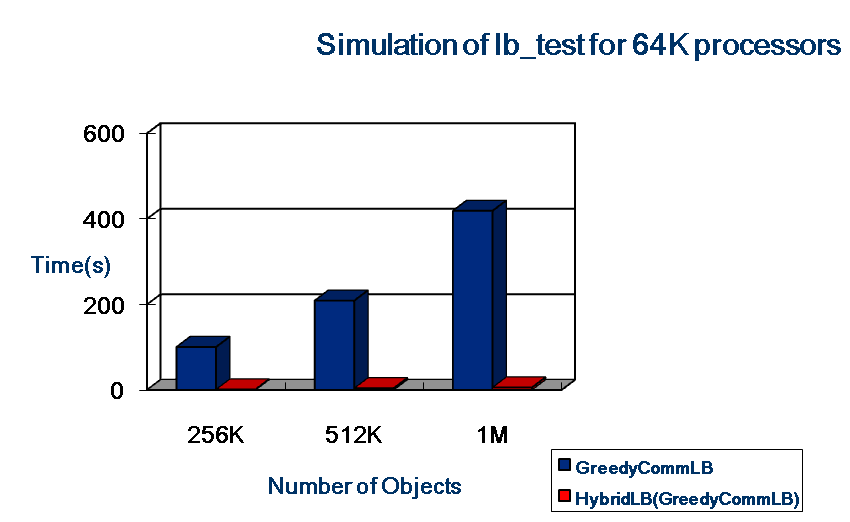
\includegraphics[width=0.5\textwidth]{figures/hybridLBPerf}
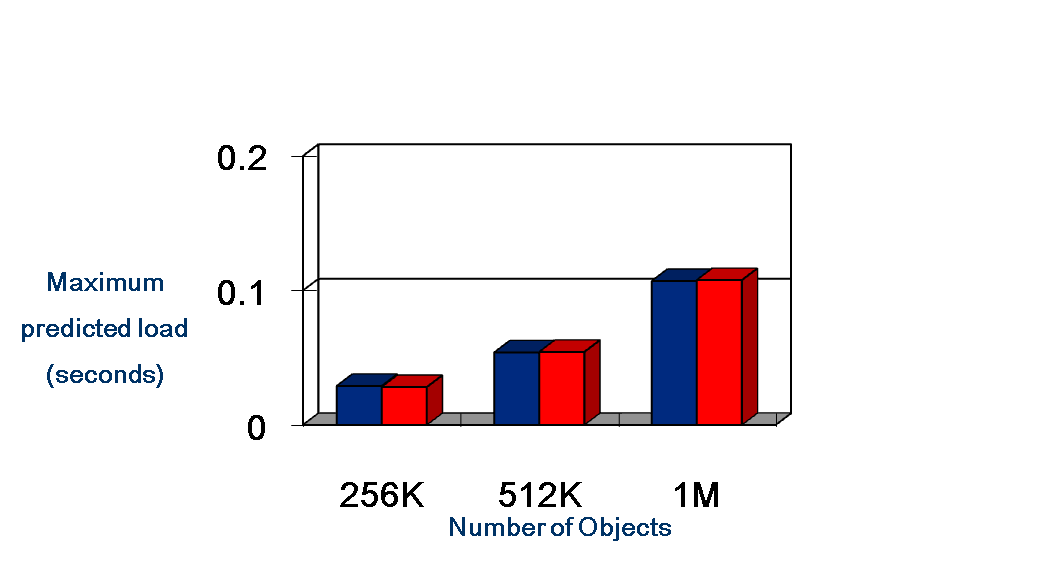
\includegraphics[width=0.5\textwidth]{figures/hybridLBquality}
\end{frame}

\begin{frame}[fragile]
\frametitle{MetaBalancer - When and how to load balance?}
\begin{itemize}    
    \item Difficult to find the optimum load balancing period
    \begin{itemize}
       \item Depends on the application characteristics
       \item Depends on the machine the application is run on
    \end{itemize}
    
    \item Monitors the application continuously and predicts behavior.
    \item Decides when to invoke which load balancer.
    \item Command line argument - \texttt{+MetaLB}
\end{itemize}
\end{frame}

\begin{frame}[fragile]
\frametitle{Metabalancer Performance for LeanMD mini-App}
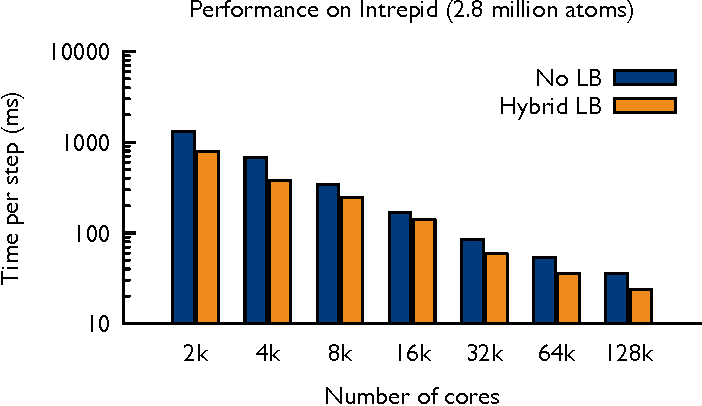
\includegraphics{figures/bgp-metabalancer-leanmd}
\end{frame}


\end{document}
